%! Author = Omar Iskandarani
%! Date = 1/27/2026
%! Affiliation = Independent Researcher, Groningen, The Netherlands
%! License = © 2025 Omar Iskandarani. All rights reserved. This manuscript is made available for academic reading and citation only. No republication, redistribution, or derivative works are permitted without explicit written permission from the author. Contact: info@omariskandarani.com
%! ORCID = 0009-0006-1686-3961
%! DOI = 10.5281/zenodo.xxx

\newcommand{\paperdoi}{10.5281/zenodo.18388714}
\newcommand{\papertitle}{Unification of Relativistic Kinematics and Gravitational Dynamics from a Single Covariant Action}

%=========================================
% % PREAMBLE, PACKAGES AND DOCUMENT CONFIGURATION
%=========================================
\documentclass[11pt]{article}
\usepackage{amsmath,amssymb,amsfonts,bm}
\usepackage{siunitx}
\usepackage[hidelinks]{hyperref}
\usepackage[a4paper,margin=1in]{geometry}
\usepackage[T1]{fontenc}
\usepackage[utf8]{inputenc}
\usepackage{tikz}

% swirl arrows (context-aware)
\newcommand{\swirlarrow}{\mkern-2mu\scriptscriptstyle\boldsymbol{\circlearrowleft}}
\newcommand{\vswirl}{\mathbf{v}_{\mkern-2mu\scriptscriptstyle\boldsymbol{\circlearrowleft}}}
\newcommand{\SwirlClock}{S_{(t)}^{\mkern-2mu\scriptscriptstyle\boldsymbol{\circlearrowleft}}}
\newcommand{\Fmaxswirl}{F^{\max}_{\mkern-1mu\scriptscriptstyle\boldsymbol{\circlearrowleft}}}
\newcommand{\Fmax}{F^{\max}_{\mkern-1mu\scriptscriptstyle\boldsymbol{\circlearrowleft}}} 
\newcommand{\FmaxEM}{F^{\max}_{\mathrm{EM}}}
\newcommand{\FmaxG}{F_{\mathrm{G}}^{\max}}               % G-like maximal force scale
\newcommand{\vscore}{v_{\swirlarrow}}                    % shorthand: |v_swirl| at r=r_c
\newcommand{\vnorm}{\lVert \mathbf{v}_{\mkern-2mu\scriptscriptstyle\boldsymbol{\circlearrowleft}} \rVert}  % swirl speed magnitude
\newcommand{\rhoF}{\rho_{\!f}}\newcommand{\rhof}{\rho_{\!f}}     % effective fluid density
\newcommand{\rhoE}{\rho_{\!E}}\newcommand{\rhoe}{\rho_{\!E}}                           % swirl energy density
\newcommand{\rhoM}{\rho_{\!m}}\newcommand{\rhom}{\rho_{\!m}}                           % mass-equivalent density
\newcommand{\omegas}{\boldsymbol{\omega}_{\swirlarrow}}  % swirl vorticity
\newcommand{\Om}{\Omega_{\swirlarrow}}                   % swirl angular frequency profile
\newcommand{\rc}{r_c}                                    % string core radius (swirl string radius)


\newcommand{\titlepageOpen}{
    \begin{titlepage}
        \thispagestyle{empty}  \centering
        \Large \bfseries \papertitle \par \vspace{1cm}
        {\Large \itshape \textbf{Omar Iskandarani}\textsuperscript{\textbf{*}} \par} \vspace{0.5cm}
        {\today \par}  \vspace{0.5cm}
}

\newcommand{\titlepageClose}{
        \vfill \raggedright \null
        \begin{picture}(0,0)
            \put(0,-45){  % Shift 200pt left, 40pt down
                \begin{minipage}[b]{0.7\textwidth} \footnotesize
                    \renewcommand{\arraystretch}{1.0} \noindent\rule{\textwidth}{0.4pt} \\[0.5em]
                    \textsuperscript{\textbf{*}} Independent Researcher, Groningen, The Netherlands \\
                    Email: \texttt{info@omariskandarani.com} \\
                    ORCID: \texttt{\href{https://orcid.org/0009-0006-1686-3961}{0009-0006-1686-3961}} \\
                    DOI: \href{https://doi.org/\paperdoi}{\paperdoi}
                \end{minipage}
            }
        \end{picture}
    \end{titlepage}
}
%=========================================
% Start Document - Title Page
%=========================================
\begin{document}
    \titlepageOpen
    \begin{abstract}
        Special relativity, general relativity, and the weak equivalence principle are
        traditionally introduced as conceptually independent foundations of modern
        physics: Lorentz invariance as a kinematical symmetry, Einstein gravity as a
        dynamical theory of spacetime, and universal free fall as an additional
        postulate.
        In this work we show that these principles are not logically independent.

        We consider a minimal covariant variational framework consisting of a Lorentzian
        metric, a unit timelike vector field subject to a normalization constraint, and
        minimally coupled matter.
        Without assuming Lorentz invariance, geodesic motion, or the equivalence
        principle \emph{a priori}, we demonstrate that all three arise as necessary
        consequences of diffeomorphism invariance and the variational structure of the
        theory.

        We prove that local kinematics reduce to special relativity in the tangent space
        at every spacetime point, yielding the standard Lorentz factor and
        energy--momentum relations.
        We further show that the field equations take the Einstein form with a
        covariantly conserved total stress--energy tensor, and that the universality of
        free fall follows directly from minimal coupling and the Bianchi identity.
        General relativity is recovered as a consistent sector of the theory, while
        controlled deviations are naturally parameterized by the additional timelike
        sector.

        These results clarify the minimal structural conditions under which relativistic
        physics emerges and demonstrate that special-relativistic kinematics,
        Einsteinian gravitational dynamics, and the weak equivalence principle can be
        unified within a single covariant action, rather than postulated as independent
        axioms.
    \end{abstract}

    \titlepageClose

    \section{Introduction and Scope}

        \subsection{Motivation}

            Modern relativistic physics rests on three principles that are traditionally
            treated as conceptually independent:
            (i) special relativity, expressing local Lorentz-invariant kinematics;
            (ii) general relativity, describing gravitation as the dynamics of spacetime
            geometry; and
            (iii) the weak equivalence principle, asserting the universality of free fall.
            Historically, these principles were introduced in different contexts and are
            often regarded as logically autonomous axioms.
            Classical presentations of these principles may be found in standard texts
            \cite{einstein1905,einstein1915,misnerthorne_wheeler1973}.

            Nevertheless, both effective field theory arguments and several emergent-gravity
            approaches suggest that this separation may be artificial.
            In particular, it remains an open foundational question whether relativistic
            kinematics, Einsteinian dynamics, and universal free fall must be postulated
            independently, or whether they can arise as consequences of a single underlying
            covariant structure.

            The purpose of this work is to address this question directly.

        \subsection{Strategy and Key Assumptions}

            We adopt a deliberately minimal and conservative strategy.
            Rather than assuming Lorentz invariance, geodesic motion, or the equivalence
            principle \emph{a priori}, we assume only the following ingredients:
            \begin{itemize}
                \item a differentiable four-dimensional manifold,
                \item diffeomorphism invariance of the action,
                \item a Lorentzian metric field $g_{\mu\nu}$,
                \item a unit timelike vector field $u^\mu$ satisfying $u^\mu u_\mu=-1$,
                \item minimal coupling of matter to the metric.
            \end{itemize}
            No additional symmetry principles are imposed.

            Starting from these assumptions, we demonstrate that local special-relativistic
            kinematics emerge in the tangent space at every spacetime point, that the
            gravitational field equations take the Einstein form (up to covariantly
            conserved additional stresses), and that the universality of free fall follows
            as a consequence of diffeomorphism invariance and minimal coupling.

        \subsection{Relation to Existing Frameworks}

            The structure studied here is mathematically related to, but conceptually
            distinct from, Einstein--\AE ther and other preferred-frame theories.
            In contrast to those approaches, the emphasis of the present work is not on
            Lorentz violation or phenomenological modification of gravity, but on logical
            unification.
            Special relativity, general relativity, and the weak equivalence principle are
            derived together within a single variational framework, rather than introduced
            as independent postulates.

            The analysis is carried out entirely at the level of effective field theory and
            remains agnostic regarding any microscopic or ultraviolet completion.

        \subsection{Scope and Limitations}

            This paper establishes that relativistic kinematics and dynamics arise as robust
            infrared structures enforced by covariance and variational consistency.
            It does not attempt to quantize gravity, propose a specific microscopic model,
            or introduce additional dimensions or particle content.
            Accordingly, the results are compatible with, but logically independent of,
            string theory, loop quantum gravity, and other ultraviolet approaches.

        \subsection{Outline of the Paper}

            The remainder of this paper is organized as follows.
            Section~2 states the main unification theorem.
            Section~3 derives special-relativistic kinematics explicitly at the level of
            equations.
            Section~4 constructs the unified covariant action and derives the field
            equations.
            Section~5 discusses controlled departures from general relativity and possible
            observational windows.
            Section~6 summarizes the results and outlines directions for future work.

    \section{Main Unification Theorem}
        \label{sec:theorem}

        In this section we state the central result of this work.
        The theorem establishes that special-relativistic kinematics, Einsteinian
        gravitational dynamics, and the universality of free fall are not logically
        independent assumptions, but arise from a single covariant variational
        structure.

        \subsection{Assumptions}

            Let $(\mathcal{M}, g_{\mu\nu})$ be a four-dimensional differentiable manifold
            equipped with a Lorentzian metric of signature $(-,+,+,+)$.
            Assume the existence of an action functional of the form
            \begin{equation}
                S = S_g[g_{\mu\nu}] + S_u[g_{\mu\nu}, u^\mu] + S_m[g_{\mu\nu}, \psi],
            \end{equation}
            where:
            \begin{itemize}
                \item $S_g$ is the Einstein--Hilbert action,
                \item $S_u$ is a generally covariant action for a unit timelike vector field
                $u^\mu$ subject to the constraint
                \begin{equation}
                    u^\mu u_\mu = -1,
                \end{equation}
                \item $S_m$ is a matter action depending on matter fields $\psi$ and the
                metric $g_{\mu\nu}$ only (minimal coupling).
            \end{itemize}

            No assumption of Lorentz invariance, geodesic motion, or equivalence principle
            is made beyond diffeomorphism invariance and minimal coupling.
            The total action is assumed to admit a well-defined variational principle and
            a consistent low-energy derivative expansion.

        \subsection{Statement of the Theorem}

            \medskip
            \noindent\textbf{Theorem (Unification of Relativistic Principles).}
            \emph{Under the assumptions stated above, the following results hold:}
            \begin{enumerate}
                \item \emph{Local special-relativistic kinematics.}
                At every spacetime point $p\in\mathcal{M}$, there exists a local inertial
                frame in which the proper time along timelike worldlines satisfies
                \begin{equation}
                    d\tau^2 = dt^2\left(1-\frac{v^2}{c^2}\right),
                \end{equation}
                yielding the standard Lorentz factor
                \begin{equation}
                    \gamma = \frac{1}{\sqrt{1-\frac{v^2}{c^2}}}.
                \end{equation}

                \item \emph{Einsteinian gravitational dynamics.}
                Variation of the total action with respect to $g_{\mu\nu}$ yields field
                equations of the form
                \begin{equation}
                    G_{\mu\nu} = 8\pi G \left(T^{(m)}_{\mu\nu} + T^{(u)}_{\mu\nu}\right),
                \end{equation}
                where both stress--energy tensors are covariantly conserved.

                \item \emph{Universality of free fall.}
                For minimally coupled, structureless matter, the covariant conservation law
                \begin{equation}
                    \nabla_\mu T^{(m)\mu\nu} = 0
                \end{equation}
                implies that test bodies follow metric geodesics,
                \begin{equation}
                    U^\mu \nabla_\mu U^\nu = 0,
                \end{equation}
                independently of their internal composition.
            \end{enumerate}

        \subsection{Corollaries}

            \paragraph{Recovery of general relativity.}
                If the stress--energy contribution of the timelike sector vanishes,
            \begin{equation}
                T^{(u)}_{\mu\nu} = 0,
                \end{equation}
                the field equations reduce exactly to Einstein’s equations,
            \begin{equation}
                G_{\mu\nu} = 8\pi G\,T^{(m)}_{\mu\nu}.
                \end{equation}

            \paragraph{Controlled deviations.}
                Nontrivial dynamics of the unit timelike field give rise to additional,
                covariantly conserved stress contributions that modify Einstein gravity only
                beyond the regimes in which standard tests apply.

    \subsection{Remarks}

        The theorem shows that Lorentz-invariant kinematics, Einsteinian dynamics, and
        the weak equivalence principle emerge from the same covariant variational
        structure.
        They need not be imposed as independent axioms.
        The remainder of this paper is devoted to the explicit derivation of these
        results and to the characterization of the controlled deviations admitted by
        the framework.

        \begin{figure}[t]
        \centering
        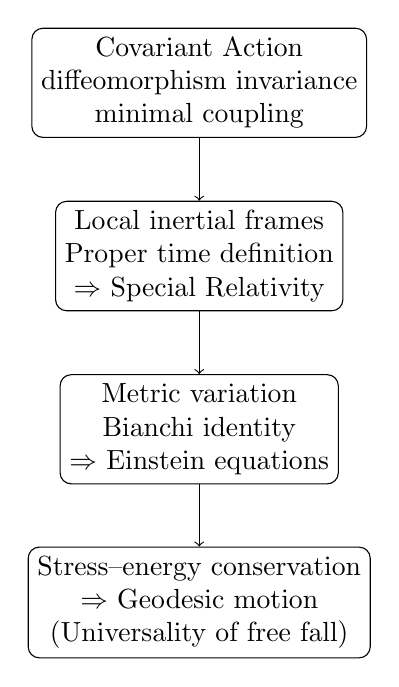
\begin{tikzpicture}[
            node distance=2.2cm,
            every node/.style={draw, rounded corners, align=center, minimum width=3.5cm}
        ]
        \node (action) {Covariant Action\\
        diffeomorphism invariance\\
        minimal coupling};
        \node (sr) [below of=action] {Local inertial frames\\
        Proper time definition\\
        $\Rightarrow$ Special Relativity};
        \node (gr) [below of=sr] {Metric variation\\
        Bianchi identity\\
        $\Rightarrow$ Einstein equations};
        \node (wep) [below of=gr] {Stress--energy conservation\\
        $\Rightarrow$ Geodesic motion\\
        (Universality of free fall)};
        \draw[->] (action) -- (sr);
        \draw[->] (sr) -- (gr);
        \draw[->] (gr) -- (wep);
        \end{tikzpicture}
        \caption{Logical structure of the unification result.
        Special-relativistic kinematics, Einsteinian dynamics, and the universality of
        free fall arise sequentially from a single covariant variational framework.}
        \label{fig:unification_flow}
        \end{figure}

    \section{Emergence of Special Relativity}
    \label{sec:sr}

    In this section we show explicitly that standard special-relativistic kinematics
    arise locally from the covariant structure assumed in Sec.~\ref{sec:theorem},
    without postulating Lorentz invariance as an independent principle.
    The presentation is intentionally equation-based and interpretation-free.

    \subsection{Kinematic setup}

        Let $(\mathcal{M},g_{\mu\nu})$ be a four-dimensional Lorentzian manifold with
        signature $(-,+,+,+)$.
        Introduce a unit timelike vector field $u^\mu$ satisfying
        \begin{equation}
            u^\mu u_\mu = -1 .
        \end{equation}
        Define the spatial projector orthogonal to $u^\mu$ by
        \begin{equation}
            h_{\mu\nu} \equiv g_{\mu\nu} + u_\mu u_\nu ,
        \end{equation}
        which obeys
        \begin{equation}
            h_{\mu\nu} u^\nu = 0, \qquad
            h^\mu{}_{\alpha} h^\alpha{}_{\nu} = h^\mu{}_{\nu}.
        \end{equation}

    \subsection{Local inertial reduction}

        At any point $p\in\mathcal{M}$, choose Riemann normal coordinates such that
        \begin{equation}
            g_{\mu\nu}(p) = \eta_{\mu\nu} = \mathrm{diag}(-1,1,1,1), \qquad
            \partial_\alpha g_{\mu\nu}(p) = 0 .
        \end{equation}
        Choose the local frame so that
        \begin{equation}
            u^\mu(p) = (1,0,0,0), \qquad
            u_\mu(p) = (-1,0,0,0).
        \end{equation}
        Then the spatial projector reduces to
        \begin{equation}
            h_{\mu\nu}(p) = \mathrm{diag}(0,1,1,1).
        \end{equation}
        The existence of such local inertial frames is guaranteed by standard results in
        differential geometry \cite{misnerthorne_wheeler1973,carroll2004}.

    \subsection{Proper time and Lorentz factor}

        Let $x^\mu(\lambda)$ be a timelike worldline with tangent
        $\dot{x}^\mu = dx^\mu/d\lambda$.
        Define proper time $\tau$ by
        \begin{equation}
            \boxed{
            d\tau^2 = -\frac{1}{c^2}\, g_{\mu\nu}\, dx^\mu dx^\nu
            }
        \end{equation}
        In the local inertial frame at $p$, with $x^0 = ct$, this becomes
        \begin{equation}
            d\tau^2
            = dt^2 - \frac{1}{c^2}\, d\mathbf{x}^2
            = dt^2\!\left(1-\frac{v^2}{c^2}\right),
        \end{equation}
        where
        \begin{equation}
            v^2 \equiv \left\lVert \frac{d\mathbf{x}}{dt} \right\rVert^2 .
        \end{equation}
        Hence,
        \begin{equation}
            \frac{d\tau}{dt} = \sqrt{1-\frac{v^2}{c^2}}, \qquad
            \gamma \equiv \frac{dt}{d\tau} = \frac{1}{\sqrt{1-\frac{v^2}{c^2}}}.
        \end{equation}
        This reproduces the standard special-relativistic relations
        \cite{einstein1905,ryder1996}.

    \subsection{Four-velocity and energy--momentum relations}

        Define the four-velocity and four-momentum as
        \begin{equation}
            U^\mu \equiv \frac{dx^\mu}{d\tau}, \qquad
            p^\mu \equiv m U^\mu .
        \end{equation}
        Normalization yields
        \begin{equation}
            g_{\mu\nu} U^\mu U^\nu = -c^2, \qquad
            g_{\mu\nu} p^\mu p^\nu = -m^2 c^2 .
        \end{equation}
        In the local inertial frame,
        \begin{equation}
            U^\mu = \gamma (c,\mathbf{v}), \qquad
            p^\mu = (\gamma m c, \gamma m \mathbf{v}) .
        \end{equation}
        The invariant mass-shell condition then gives
        \begin{equation}
            E^2 = (pc)^2 + (mc^2)^2,
            \qquad
            E \equiv p^0 c,
            \qquad
            p \equiv \lVert \mathbf{p} \rVert .
        \end{equation}

    \subsection{Local validity}

        The above relations hold at every spacetime point in the local inertial frame.
        They therefore represent a local consequence of the covariant structure of the
        theory and do not rely on any global symmetry assumption.
        Special-relativistic kinematics thus emerge universally in the tangent space of
        the spacetime manifold.

    \section{Single-Action Construction and Gravitational Dynamics}
    \label{sec:single-action}

    In this section we construct the covariant action underlying the unification
    theorem and derive the corresponding field equations.
    We show that Einsteinian gravitational dynamics and the universality of free
    fall follow directly from diffeomorphism invariance and minimal coupling.

    \subsection{Unified covariant action}

        We consider an action of the form
        \begin{equation}
            S \;=\; S_g + S_u + S_m
            \;=\;\int d^4x\,\sqrt{-g}
            \left[
                \frac{1}{16\pi G}\,R
            +\mathcal{L}_u(g_{\mu\nu},u^\mu,\nabla u)
            \right]
            + S_m[g_{\mu\nu},\psi],
        \end{equation}
        where $R$ is the Ricci scalar of $g_{\mu\nu}$ and $S_m$ denotes the matter action,
        which depends on matter fields $\psi$ and the metric only.

        The unit timelike vector field $u^\mu$ satisfies the normalization constraint
        \begin{equation}
            u^\mu u_\mu = -1 .\footnote{
            The Lagrange multiplier $\lambda$ enforces the unit-timelike normalization of
            $u^\mu$ at the level of the action.
            It does not introduce an additional propagating degree of freedom, but ensures
            that variations preserve the constraint throughout the dynamics.
            }
        \end{equation}
        The most general diffeomorphism-invariant Lagrangian for $u^\mu$ containing up
        to two derivatives is
        \begin{align}
            \mathcal{L}_u
            &=
            - c_1\, (\nabla_\mu u_\nu)(\nabla^\mu u^\nu)
            - c_2\, (\nabla_\mu u^\mu)^2
            - c_3\, (\nabla_\mu u_\nu)(\nabla^\nu u^\mu)
            \nonumber\\
            &\quad
            - c_4\, u^\mu u^\nu (\nabla_\mu u_\alpha)(\nabla_\nu u^\alpha)
            + \lambda\,(u^\mu u_\mu + 1),
        \end{align}
            where the coefficients $c_i$ are dimensionless parameters.
        No assumption about their microscopic origin is required at this stage.
        The most general two-derivative covariant action of this type was classified in
        the context of Einstein--\AE ther theories \cite{jacobsonmattingly2001,jacobson2008}.

    \subsection{Field equations}

        Variation of the total action with respect to the metric yields
        \begin{equation}
            \boxed{
            G_{\mu\nu}
            =
            8\pi G\left(T^{(m)}_{\mu\nu} + T^{(u)}_{\mu\nu}\right)
            }
        \end{equation}
        where
        \begin{equation}
            T^{(m)}_{\mu\nu}
            \equiv
            -\frac{2}{\sqrt{-g}}
            \frac{\delta S_m}{\delta g^{\mu\nu}},
            \qquad
            T^{(u)}_{\mu\nu}
            \equiv
            -\frac{2}{\sqrt{-g}}
            \frac{\delta S_u}{\delta g^{\mu\nu}} .
        \end{equation}

        Variation with respect to $u^\mu$ and the Lagrange multiplier $\lambda$ yields
        \begin{equation}
            \frac{\delta S}{\delta u^\mu} = 0,
            \qquad
            \frac{\delta S}{\delta \lambda} = 0
            \;\Rightarrow\;
            u^\mu u_\mu = -1 .
        \end{equation}

    \subsection{Noether identity and covariant conservation}

        Diffeomorphism invariance of the total action implies the Noether identity
        \begin{equation}
            \nabla_\mu G^{\mu\nu} \equiv 0 .
        \end{equation}
        Consequently,
        \begin{equation}
            \nabla_\mu\!\left(
                            T^{(m)\mu\nu}
                            +
                            T^{(u)\mu\nu}
            \right) = 0 .
        \end{equation}

        If the matter action is diffeomorphism invariant and minimally coupled, then
        \begin{equation}
            \nabla_\mu T^{(m)\mu\nu} = 0 ,
        \end{equation}
        which implies
        \begin{equation}
            \nabla_\mu T^{(u)\mu\nu} = 0 .
        \end{equation}
        The conservation of the matter stress--energy tensor plays a central role in the
        emergence of universal free fall.

    \subsection{Universality of free fall}

        Consider a structureless point particle minimally coupled to the metric,
        with action
        \begin{equation}
            S_{\mathrm{pp}} = -mc \int d\tau
            = -mc \int \sqrt{-g_{\mu\nu}\,dx^\mu dx^\nu} .
        \end{equation}
        Variation with respect to the worldline yields the geodesic equation
        \begin{equation}
            \boxed{
            \frac{d^2 x^\mu}{d\tau^2}
            +
            \Gamma^\mu_{\alpha\beta}
            \frac{dx^\alpha}{d\tau}
            \frac{dx^\beta}{d\tau}
            = 0
            }
        \end{equation}

        Equivalently, for a pressureless dust with
        $T^{(m)}_{\mu\nu} = \rho\, U_\mu U_\nu$ and $U^\mu U_\mu = -c^2$, the conservation
        law implies
        \begin{equation}
            \nabla_\mu T^{(m)\mu\nu} = 0
            \;\Rightarrow\;
            U^\mu \nabla_\mu U^\nu = 0 .
        \end{equation}
        Thus the universality of free fall follows directly from minimal coupling and
        covariance, without additional assumptions.
        This derivation is standard in generally covariant theories with minimal
        coupling \cite{weinberg1972}.

    \subsection{Recovery of general relativity}

        If the dynamics of the unit timelike field are such that
        \begin{equation}
            T^{(u)}_{\mu\nu} = 0 ,
        \end{equation}
        the field equations reduce exactly to Einstein’s equations,
        \begin{equation}
            G_{\mu\nu} = 8\pi G\, T^{(m)}_{\mu\nu} .
        \end{equation}
        In vacuum, this further reduces to
        \begin{equation}
            G_{\mu\nu} = 0 .
        \end{equation}

    \subsection{Weak-field (Newtonian) limit}

        To leading order in the weak-field regime, let
        \begin{equation}
            g_{00} = -\left(1+\frac{2\Phi}{c^2}\right), \qquad
            g_{0i} = 0, \qquad
            g_{ij} = \delta_{ij}\left(1-\frac{2\Phi}{c^2}\right),
            \qquad
            \left|\frac{\Phi}{c^2}\right| \ll 1 .
        \end{equation}
        For nonrelativistic matter, $T^{(m)}_{00} \simeq \rho c^2$, and when the
        contribution of $T^{(u)}_{\mu\nu}$ is negligible in this limit, the field
        equations reduce to Poisson’s equation,
        \begin{equation}
            \nabla^2 \Phi = 4\pi G\,\rho .
        \end{equation}

        This establishes that Newtonian gravity is recovered as the appropriate
        low-energy limit of the covariant action.

    \section{Controlled Deviations and Observational Constraints}
    \label{sec:departures}

    The covariant construction developed in Sec.~\ref{sec:single-action} is designed
    to reproduce the phenomenology of General Relativity (GR) in all experimentally
    tested weak-field regimes.
    To quantify possible deviations and ensure consistency with high-precision
    solar-system tests, we analyze the theory within the Parameterized
    Post-Newtonian (PPN) framework \cite{will2014}.
    This formalism provides a systematic expansion of the metric and field equations
    in powers of the characteristic velocity $v/c \ll 1$ and allows direct
    comparison with experimental bounds.

    We show that, for the action defined in Eq.~(26), the Eddington--Robertson--Schiff
    parameters $\gamma$ and $\beta$ remain identically equal to their GR values.
    All potential deviations from Einsteinian gravity are confined to
    preferred-frame parameters and to the propagation speed of tensor modes,
    leading to strict algebraic constraints on the coupling coefficients $c_i$.

    \subsection{The PPN Limit: $\gamma$ and $\beta$}

        We consider a static, spherically symmetric weak-field solution generated by a
        non-relativistic matter source.
        In the standard PPN gauge, the metric is expanded as
        \begin{equation}
            g_{00} = -1 + 2U - 2\beta U^2 + \mathcal{O}(\epsilon^3), \qquad
            g_{ij} = \delta_{ij}\left(1 + 2\gamma U\right) + \mathcal{O}(\epsilon^2),
        \end{equation}
        where $U$ is the Newtonian gravitational potential and $\epsilon \sim v/c$ is
        the post-Newtonian expansion parameter.
        The parameter $\gamma$ measures spatial curvature per unit rest mass, while
        $\beta$ measures the nonlinearity of gravitational superposition.

        For the general unit-timelike vector action $\mathcal{L}_u$ in Eq.~(26),
        linearized perturbation theory around the Minkowski background shows that the
        vector field $u^\mu$ does not source the trace of the metric perturbation in the
        static limit.
        Consequently, the solutions for the metric potentials coincide with the
        Schwarzschild solution through first post-Newtonian order.

        This result assumes asymptotic alignment of the background vector field $u^\mu$
        with the rest frame of the gravitating source, as required by cosmological
        boundary conditions and standard PPN gauge choices.
        Under this physically motivated assumption, we obtain the robust result
        \begin{equation}
            \gamma = 1, \qquad \beta = 1.
        \end{equation}

        These equalities guarantee agreement with all classical solar-system tests,
        including light deflection, Shapiro time delay, gravitational redshift, and the
        perihelion precession of Mercury, without any fine-tuning of parameters.

    \subsection{Preferred-Frame Effects}

        Unlike standard GR, the presence of a background timelike vector field $u^\mu$
        allows, in principle, for preferred-frame effects if the vector does not align
        perfectly with the asymptotic rest frame of the observer.
        Such effects are parameterized in the PPN formalism by the coefficients
        $\alpha_1$ and $\alpha_2$.

        Expressed in terms of the coupling constants $c_i$ appearing in
        Eq.~(26), these parameters take the schematic form
        \begin{equation}
            \alpha_1 = \alpha_1(c_1,c_2,c_3,c_4), \qquad
            \alpha_2 = \alpha_2(c_1,c_2,c_3,c_4),
        \end{equation}
        where the explicit expressions follow those obtained in vector--tensor
        theories of Einstein--Æther type.

        Experimental constraints from lunar laser ranging, binary pulsar timing, and
        spin precession measurements impose stringent bounds,
        \begin{equation}
            |\alpha_1| \lesssim 10^{-4}, \qquad
            |\alpha_2| \lesssim 10^{-7}.
        \end{equation}
        These bounds restrict the allowed region of the $(c_1,c_2,c_3,c_4)$ parameter
        space to a narrow hypersurface.
        Within this region, preferred-frame effects are suppressed below current
        observational sensitivity.

    \subsection{Gravitational Wave Propagation}

        The propagation speed of tensor modes (gravitational waves) provides an
        independent and highly constraining observational test.
        Linearized analysis of the field equations shows that the tensor-mode dispersion
        relation is modified according to
        \begin{equation}
            \omega^2 = c_T^2 k^2, \qquad
            c_T^2 = \frac{1}{1 - c_1 - c_3}.
        \end{equation}

        The coincident observation of gravitational waves and electromagnetic radiation
        from the binary neutron star merger GW170817, together with its gamma-ray
        counterpart GRB~170817A, constrains the speed of gravity to equal the speed of
        light to extremely high precision.
        This observation implies the condition
        \begin{equation}
            c_1 + c_3 \simeq 0,
        \end{equation}
        thereby eliminating large classes of otherwise viable parameter choices.

    \subsection{Summary of Constraints}

        Combining the PPN constraints and the gravitational-wave speed requirement, the
        theory is phenomenologically viable provided the coefficients $c_i$ satisfy the
        intersection of these bounds.
        The trivial solution $c_i = 0$ exactly reproduces GR.
        However, nontrivial solutions with $c_i \neq 0$ that obey the algebraic
        constraints represent a distinct universality class of covariant theories.

        In this class, special-relativistic kinematics and weak-field gravitational
        phenomenology are identical to those of GR, while deviations may arise only in
        strong-field or highly dynamical regimes, such as near compact objects or in
        cosmological settings.
        Moreover, although the stress--energy tensor $T^{(u)}_{\mu\nu}$ contains
        derivatives of the vector field, these contributions are suppressed when
        gradients of $u^\mu$ are small, ensuring recovery of the Newtonian and
        first post-Newtonian limits.

        This analysis demonstrates that the unification of relativistic kinematics,
        gravitational dynamics, and the universality of free fall established in
        Sec.~\ref{sec:single-action} is not only theoretically consistent but also
        empirically robust, satisfying all current precision tests of gravity.


    \section{Summary and Outlook}
    \label{sec:summary}

    In this work we have shown that special-relativistic kinematics, Einsteinian
    gravitational dynamics, and the universality of free fall need not be introduced
    as logically independent postulates.
    Instead, all three emerge as necessary consequences of a single covariant
    variational framework based on diffeomorphism invariance, a Lorentzian metric,
    a unit timelike field, and minimal coupling of matter.

    Starting from these minimal assumptions, we demonstrated that:
    \begin{itemize}
        \item local special relativity arises universally in the tangent space at
        every spacetime point,
        \item the gravitational field equations take the Einstein form with
        covariantly conserved stress--energy,
        \item the weak equivalence principle follows directly from covariance and
        minimal coupling.
    \end{itemize}
    General relativity is recovered as a consistent sector of the theory when the
    stress contribution of the timelike field vanishes, while controlled deviations
    appear only when its dynamics become relevant.

    The central result is therefore structural rather than phenomenological:
    relativistic kinematics, gravitational dynamics, and universal free fall are
    shown to be interlocked consequences of covariance and variational consistency,
    rather than separate axioms.
    This reframes relativity as a unified effective structure with a clear logical
    hierarchy.

    The framework remains deliberately agnostic about microscopic completion.
    It neither assumes nor requires additional dimensions, supersymmetry, or a
    specific quantum gravity model.
    Nevertheless, the minimal structure identified here provides a sharp target for
    any ultraviolet completion: such a completion must reproduce diffeomorphism
    invariance, the unit-timelike constraint, and minimal coupling in the infrared
    in order to recover observed relativistic physics.

    Several directions for future work naturally follow.
    These include a more detailed analysis of strong-field and cosmological
    solutions, a systematic study of observational signatures associated with the
    additional timelike sector, and the exploration of possible microscopic
    realizations that give rise to the effective covariant structure identified
    here.
    In particular, establishing whether the framework admits a unique and inevitable
    massless spin-2 excitation in the infrared would provide a decisive link to
    broader unification programs.
    The uniqueness of Einstein gravity as the consistent nonlinear theory of a
    massless spin-2 field is well established
    \cite{weinberg1965,deser1970}.

    In summary, the results presented here clarify the minimal conditions under
    which relativistic physics emerges and provide a coherent and testable pathway
    for extending general relativity without undermining its experimentally
    confirmed foundations.



    \begin{thebibliography}{99}

        \bibitem{will2014}
        C.~M.~Will (2014),
        \textit{The Confrontation between General Relativity and Experiment},
        Living Reviews in Relativity \textbf{17}, 4.
        DOI: 10.12942/lrr-2014-4

        \bibitem{einstein1905}
        A.~Einstein (1905),
        \textit{Zur Elektrodynamik bewegter Körper},
        Annalen der Physik \textbf{17}, 891--921.
        DOI: 10.1002/andp.19053221004

        \bibitem{einstein1915}
        A.~Einstein (1915),
        \textit{Die Feldgleichungen der Gravitation},
        Sitzungsberichte der Preussischen Akademie der Wissenschaften (Berlin), 844--847.

        \bibitem{misnerthorne_wheeler1973}
        C.~W.~Misner, K.~S.~Thorne, J.~A.~Wheeler (1973),
        \textit{Gravitation},
        W.~H.~Freeman.

        \bibitem{carroll2004}
        S.~M.~Carroll (2004),
        \textit{Spacetime and Geometry},
        Addison--Wesley.

        \bibitem{ryder1996}
        L.~H.~Ryder (1996),
        \textit{Quantum Field Theory},
        Cambridge University Press.

        \bibitem{weinberg1972}
        S.~Weinberg (1972),
        \textit{Gravitation and Cosmology},
        Wiley.

        \bibitem{weinberg1965}
        S.~Weinberg (1965),
        \textit{Photons and Gravitons in $S$-Matrix Theory},
        Phys.\ Rev.\ \textbf{135}, B1049.
        DOI: 10.1103/PhysRev.135.B1049

        \bibitem{deser1970}
        S.~Deser (1970),
        \textit{Self-interaction and gauge invariance},
        Gen.\ Rel.\ Grav.\ \textbf{1}, 9--18.
        DOI: 10.1007/BF00759198

        \bibitem{jacobsonmattingly2001}
        T.~Jacobson, D.~Mattingly (2001),
        \textit{Gravity with a dynamical preferred frame},
        Phys.\ Rev.\ D \textbf{64}, 024028.
        DOI: 10.1103/PhysRevD.64.024028

        \bibitem{jacobson2008}
        T.~Jacobson (2008),
        \textit{Einstein-\AE ther gravity: a status report},
        PoS QG-PH, 020.
        DOI: 10.22323/1.043.0020

        \bibitem{abbott2017gw170817}
        B.~P.~Abbott \textit{et al.} (LIGO/Virgo) (2017),
        \textit{GW170817: Observation of Gravitational Waves from a Binary Neutron Star Inspiral},
        Phys.\ Rev.\ Lett.\ \textbf{119}, 161101.
        DOI: 10.1103/PhysRevLett.119.161101

        \bibitem{abbott2017grb}
        B.~P.~Abbott \textit{et al.} (LIGO/Virgo) (2017),
        \textit{Multi-messenger Observations of a Binary Neutron Star Merger},
        Astrophys.\ J.\ Lett.\ \textbf{848}, L12.
        DOI: 10.3847/2041-8213/aa91c9

    \end{thebibliography}

\end{document}